\documentclass[aspectratio=169,11pt]{beamer}
% ==========================================================================
%  KSA lecture-slide theme  =  stock beamer "Boadilla"  +  KSA colour theme
%  brand colours sampled from the official KSA symbol mark:
%    Deep Prussian Blue  #2E3192   (지성 - intellect)
%    Golden Gray         #D6CBB1   (감성 - sensibility)
%  Engine: XeLaTeX.  Usage:
%    \documentclass[aspectratio=169,11pt]{beamer}
%    \input{../../theme/ksa-theme.tex}
%  Each deck lives in its own slides/kor/<deck>/ folder together with its
%  own images; ../../figs/ is kept only as a fallback for the shared cache.
% ==========================================================================

\usepackage{fontspec}
\usepackage{amsmath,amssymb}
\usepackage{graphicx}
\graphicspath{{figs/}{./}{../../../figs/}}
\usepackage{booktabs}
\usepackage{listings}
\usepackage{varwidth}

% ---- fonts (no ctex/xeCJK on this box -> fontspec drives CJK directly) -----
\defaultfontfeatures{Ligatures=TeX}
\setmainfont{Noto Sans CJK KR}
\setsansfont{Noto Sans CJK KR}
\setmonofont{Noto Sans Mono CJK KR}[Scale=0.92]

% ---- base theme: stock Boadilla ------------------------------------------
\usetheme{Boadilla}
\usefonttheme{professionalfonts}
\setbeamertemplate{navigation symbols}{}

% ---- KSA colour theme (recolour the stock theme) --------------------------
\definecolor{ksablue}{HTML}{2E3192}
\definecolor{ksabluedk}{HTML}{20226A}
\definecolor{ksagold}{HTML}{D6CBB1}
\definecolor{ksagolddk}{HTML}{A9976B}
\definecolor{ksared}{HTML}{C0392B}
\definecolor{ksagray}{HTML}{5B5B5B}

\setbeamercolor{structure}{fg=ksablue}
\setbeamercolor{alerted text}{fg=ksared}

\setbeamercolor{palette primary}{fg=white,           bg=ksablue}
\setbeamercolor{palette secondary}{fg=white,         bg=ksablue!85!black}
\setbeamercolor{palette tertiary}{fg=white,          bg=ksabluedk}
\setbeamercolor{titlelike}{fg=ksablue}
\setbeamercolor{frametitle}{fg=ksablue,bg=}
\setbeamercolor{title}{fg=ksablue}
\setbeamercolor{author}{fg=ksagray}
\setbeamercolor{institute}{fg=ksagray}
\setbeamercolor{block title}{fg=white,bg=ksablue}
\setbeamercolor{block body}{fg=black!85,bg=ksablue!6}
\setbeamercolor{item}{fg=ksablue}
\setbeamercolor{section in toc}{fg=black!85}

\setbeamerfont{frametitle}{series=\bfseries}
\setbeamerfont{title}{series=\bfseries}

% ---- footline:  KSA mark | "Made by ..." | n / N   (matches reference) ----
\newcommand{\ksacredit}{}
\setbeamertemplate{footline}{%
  \hbox{%
    \begin{beamercolorbox}[wd=.18\paperwidth,ht=2.6ex,dp=1.5ex,leftskip=1.1em]{}%
      \raisebox{-0.35ex}{\includegraphics[height=2.0ex]{ksa-logo.png}}%
    \end{beamercolorbox}%
    \begin{beamercolorbox}[wd=.64\paperwidth,ht=2.6ex,dp=1.5ex,center]{}%
      {\scriptsize\color{ksagray}\ksacredit}%
    \end{beamercolorbox}%
    \begin{beamercolorbox}[wd=.18\paperwidth,ht=2.6ex,dp=1.5ex,rightskip=1.1em]{}%
      \hfill{\scriptsize\color{ksablue}\insertframenumber\,/\,\inserttotalframenumber}%
    \end{beamercolorbox}%
  }%
  \vskip2pt
}

% ---- section divider: stock \sectionpage, KSA-coloured -------------------
\setbeamertemplate{section page}{%
  \begingroup\centering
    {\color{ksagolddk}\rule{0.16\paperwidth}{1pt}}\par\vskip1.0em
    {\usebeamerfont{title}\color{ksablue}\insertsectionhead\par}\vskip1.0em
    {\color{ksagolddk}\rule{0.16\paperwidth}{1pt}}\par
  \endgroup
}
\AtBeginSection[]{\begin{frame}[plain,noframenumbering]\vfill\sectionpage\vfill\end{frame}}

% ---- code listings ------------------------------------------------------------
\lstdefinestyle{ksa}{%
  basicstyle=\ttfamily\scriptsize,
  keywordstyle=\color{ksablue}\bfseries,
  commentstyle=\color{ksagray}\itshape,
  stringstyle=\color{ksagolddk},
  numberstyle=\tiny\color{ksagray},
  backgroundcolor=\color{ksablue!6},
  frame=leftline, framerule=1.4pt, rulecolor=\color{ksablue},
  xleftmargin=1em, aboveskip=0.8em, belowskip=0.4em,
  showstringspaces=false, breaklines=true, language=Python,
}
\lstset{style=ksa}

% ---- handy macros -----------------------------------------------------------
\newcommand{\kb}[1]{\textbf{\color{ksablue}#1}}   % blue keyword
\newcommand{\kq}[1]{\textbf{\color{ksared}#1}}    % red key-question

\setbeamerfont{title}{series=\bfseries,size=\fontsize{24}{30}\selectfont}
\setbeamerfont{subtitle}{series=\bfseries,size=\fontsize{14}{18}\selectfont}
\setbeamerfont{author}{size=\normalsize}
\setbeamerfont{institute}{size=\small}
\graphicspath{{figs/}{../../../../assets/}}
\makeatletter
\newcommand{\markpage}[1]{\protected@write\@auxout{}{\string\newlabel{#1}{{\the\c@framenumber}{}}}\hypertarget{#1}{}}
\newcommand{\pref}[1]{\hyperlink{#1}{\textcolor{ksagolddk}{(p.\ref{#1})}}}
\makeatother

\renewcommand{\ksacredit}{Machine Learning 1 \,\textperiodcentered\, Early Stopping}
\title{Early Stopping (조기 종료)}
\subtitle{오래 학습한다고 좋은 모델이 되지는 않는다}
\author{Machine Learning 1}
\institute{한국과학영재학교 (KSA)}
\date{}
\begin{document}
\begin{frame}[plain,noframenumbering]\titlepage\end{frame}

% --- 오늘의 질문
\begin{frame}{오늘의 질문}
\vfill
\centering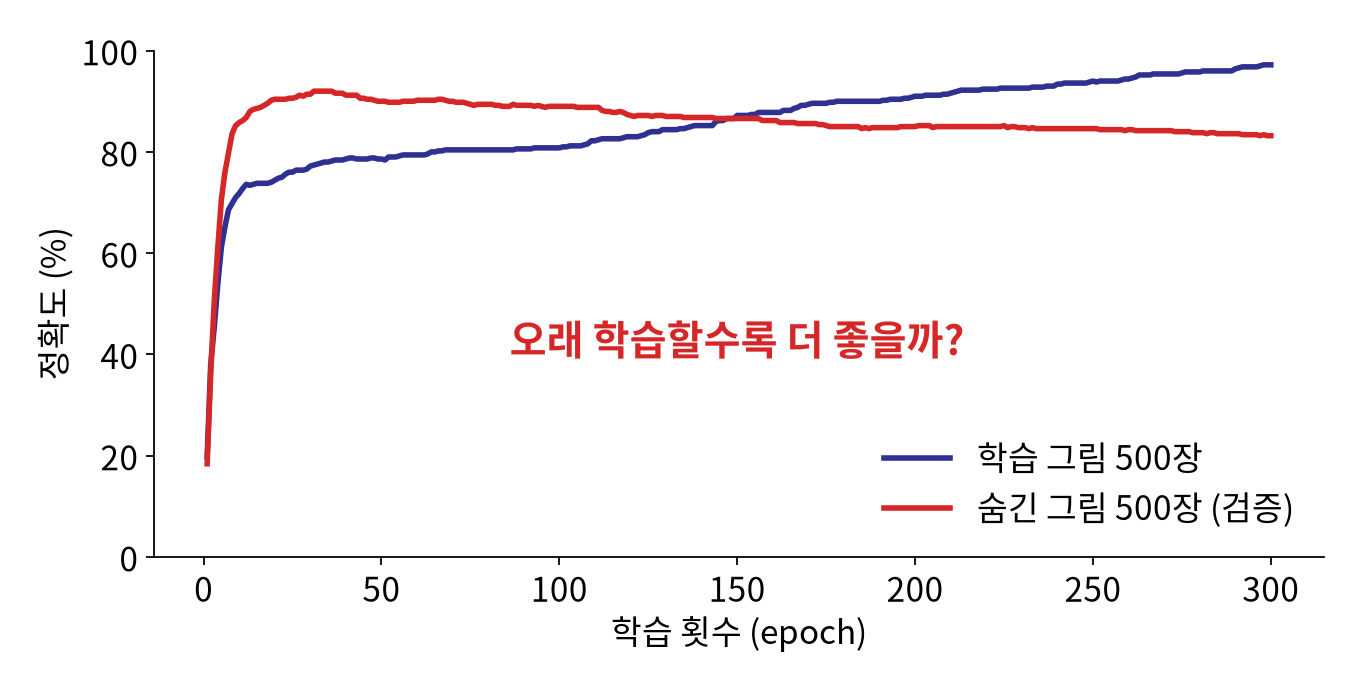
\includegraphics[width=0.64\linewidth]{es_hook.png}\par\vskip0.2em
{\large 신경망을 300번 학습했다. 파랑은 계속 오르는데 빨강은? \kq{언제 멈춰야 할까?}}
\vfill
\note{손글씨 숫자를 읽는 작은 신경망을 300번 학습했습니다. 파란 선은 학습에 쓴 그림의 정확도인데 계속 오릅니다. 빨간 선은 학습에 쓰지 않고 숨겨 둔 그림의 정확도입니다. 처음엔 같이 오르다가 어느 순간부터 내려갑니다. 오래 학습할수록 좋은 게 아니라는 뜻입니다. 그러면 언제 멈춰야 할까요? 오늘은 그 답, Early Stopping을 배웁니다.}
\end{frame}

% --- 실험
\begin{frame}{실험: 손글씨 숫자 500장}
\vfill
\centering
\renewcommand{\arraystretch}{1.5}
{\large\begin{tabular}{ll}
데이터 & 손글씨 숫자 그림 (8 × 8 픽셀, scikit-learn \texttt{load\_digits})\\
학습 & \textbf{500장} \quad 그중 20\% (100장) 의 정답을 일부러 다른 숫자로 바꿔 둠\\
검증 & 다른 \textbf{500장}, 학습에 쓰지 않고 숨겨 둔다 (정답은 그대로)\\
모델 & 작은 신경망 (은닉층 1개, 뉴런 256개), 한 번 (epoch) 씩 300번 학습
\end{tabular}}\vskip0.6em
{\small 정답을 일부러 틀리게 한 이유: 실제 데이터의 라벨 실수를 흉내 내고, 과대적합이 잘 보이게 하려고}
\vfill
\note{실험 조건입니다. scikit-learn에 들어 있는 8 곱하기 8 픽셀 손글씨 숫자 그림을 씁니다. 500장으로 학습하고, 다른 500장은 숨겨 둡니다. 이게 검증 데이터입니다. 하나 덧붙이면, 학습 그림 500장 중 100장은 정답을 일부러 다른 숫자로 바꿔 놓았습니다. 실제 데이터에도 사람이 라벨을 잘못 붙인 실수가 섞여 있는데, 그걸 흉내 내고 과대적합이 잘 보이게 하려는 겁니다. 검증 그림의 정답은 그대로입니다. 모델은 은닉층 하나에 뉴런 256개인 작은 신경망이고, 데이터 전체를 한 번 보는 걸 한 번의 학습, epoch이라고 부릅니다.}
\end{frame}

% --- 곡선
\begin{frame}{31번째에 검증 92\%, 300번째에는 83\%}
\markpage{curve}
\vfill
\centering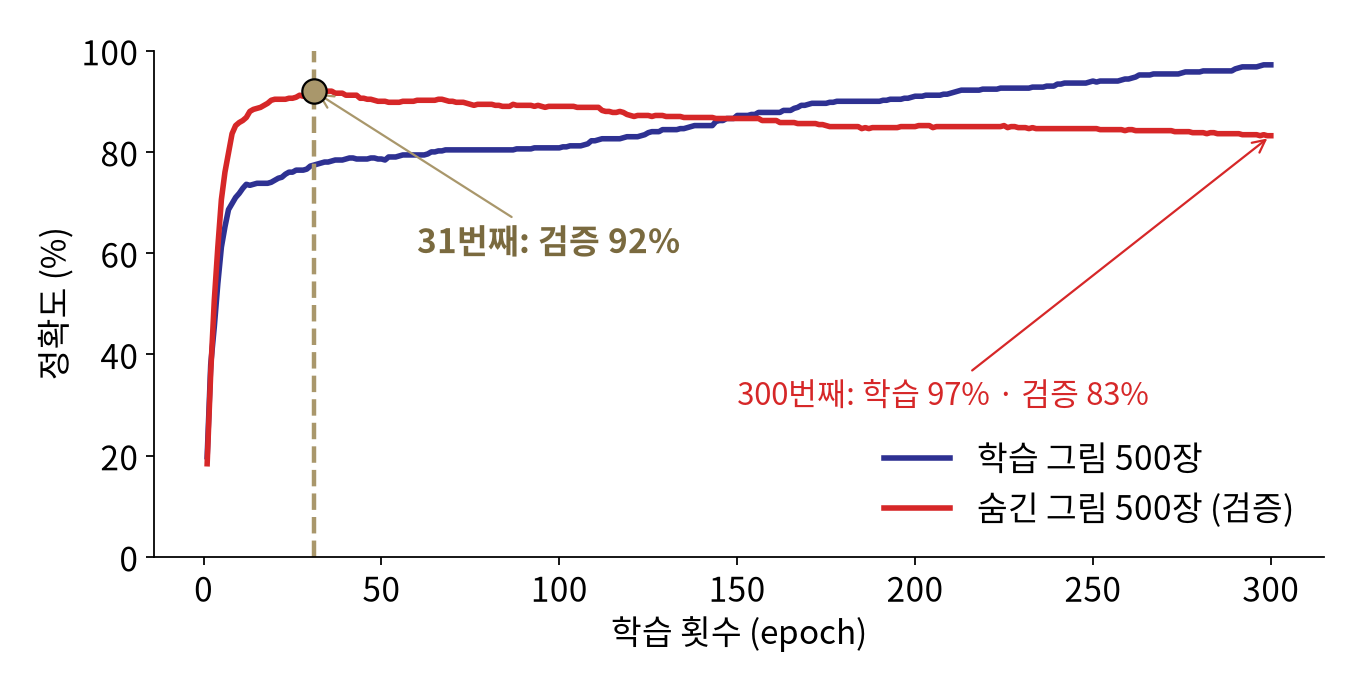
\includegraphics[width=0.66\linewidth]{es_curve.png}\par\vskip0.2em
{\large 학습: 77\% $\to$ \textbf{97\%} \qquad 검증: \kb{92\%} $\to$ \kq{83\%} \qquad (31번째 $\to$ 300번째)}
\vfill
\note{결과입니다. 31번째 학습에서 숨긴 그림을 92퍼센트 맞혀 가장 높습니다. 이때 학습 그림 정확도는 77퍼센트입니다. 정답을 일부러 바꾼 20퍼센트를 따라 하지 않았으니 80퍼센트 근처가 자연스럽습니다. 계속 학습하면 학습 정확도는 300번째에 97퍼센트까지 오릅니다. 그런데 검증 정확도는 92에서 83퍼센트로 떨어집니다. 학습 그림만 잘 맞히고 처음 보는 그림은 못 맞히는 과대적합입니다.}
\end{frame}

% --- 외움
\begin{frame}{무엇이 일어났나: 틀린 정답까지 외웠다}
\vfill
\centering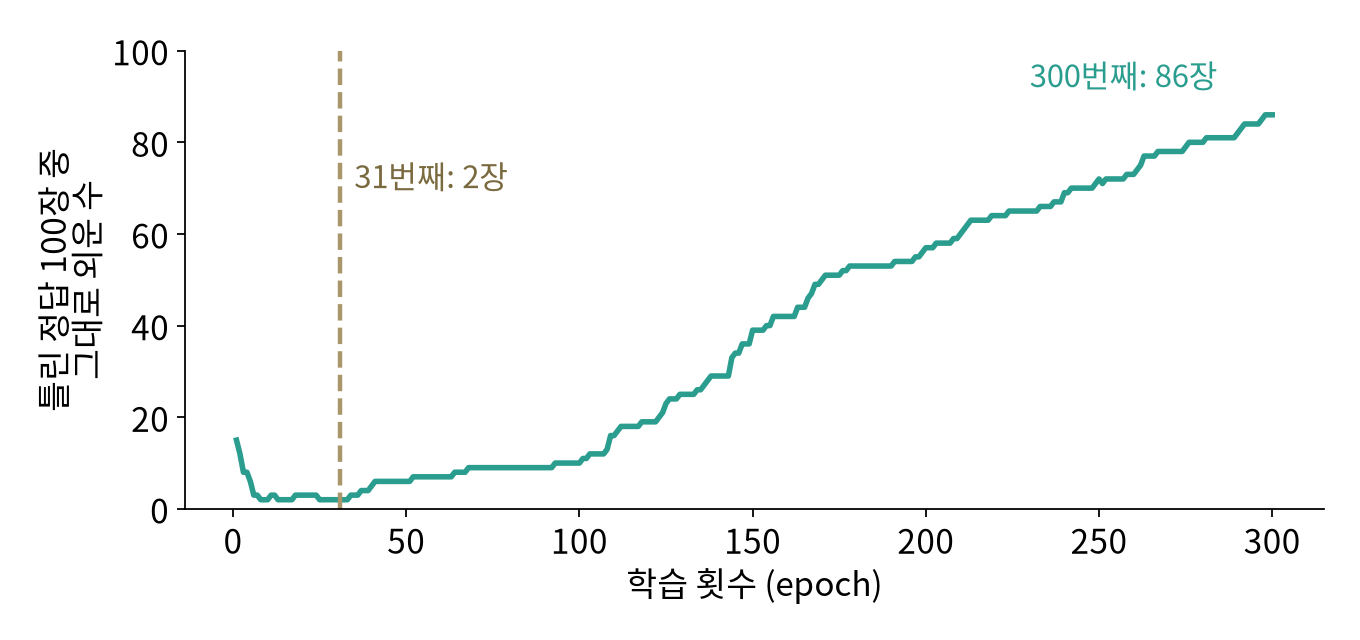
\includegraphics[width=0.62\linewidth]{es_mem.png}\par\vskip0.2em
{\large 틀리게 적은 정답 100장 중 \textbf{그대로 따라 답한} 수: \; 31번째 \kb{2장} $\to$ 300번째 \kq{86장}}
\vfill
\note{왜 그럴까요? 정답을 일부러 틀리게 적은 학습 그림 100장을 봅니다. 예를 들어 3인 그림에 정답이 7이라고 적혀 있습니다. 31번째까지는 모델이 이런 그림에도 진짜 숫자인 3이라고 답했고, 틀린 정답을 따라 한 건 2장뿐입니다. 숫자의 일반적인 모양을 배웠기 때문입니다. 그런데 계속 학습하면 학습 정확도를 올리려고 이 틀린 정답까지 하나하나 외웁니다. 300번째에는 100장 중 86장을 틀린 정답 그대로 답합니다. 학습 정확도 97퍼센트는 이렇게 얻은 것입니다.}
\end{frame}

% --- 맞히던 그림
\begin{frame}{외운 대가: 맞히던 그림을 틀린다}
\vfill
\centering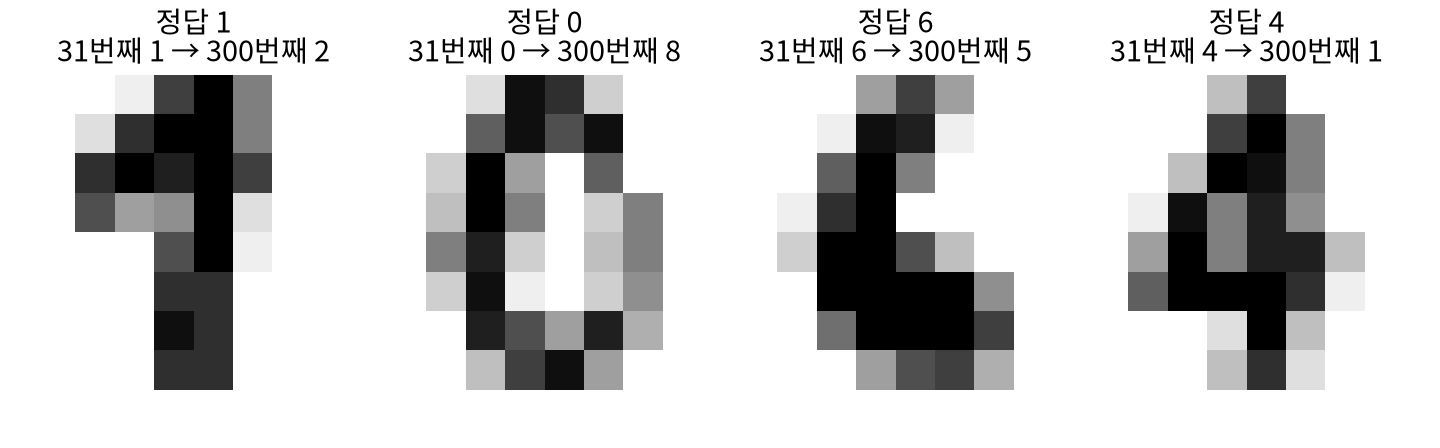
\includegraphics[width=0.66\linewidth]{es_digits.png}\par\vskip0.3em
{\large 31번째엔 맞히다가 300번째엔 틀린 검증 그림: \kq{59장}}\\[0.3em]
{\small 이상한 예외를 외우느라 경계가 구불구불해져서, 멀쩡한 1 을 2 로, 0 을 8 로 읽는다}
\vfill
\note{틀린 정답을 외운 대가는 검증 그림에서 나타납니다. 31번째에는 맞혔는데 300번째에는 틀리게 된 검증 그림이 59장입니다. 멀쩡한 1을 2로, 0을 8로, 6을 5로, 4를 1로 읽습니다. 틀린 정답이 붙은 예외들을 맞히느라 숫자 사이의 경계가 구불구불해졌고, 그 구불구불한 경계에 정상적인 그림이 걸린 겁니다.}
\end{frame}

% --- 조기 종료
\begin{frame}{Early Stopping: 검증 정확도가 가장 높을 때 멈춘다}
\markpage{es}
\vfill
\centering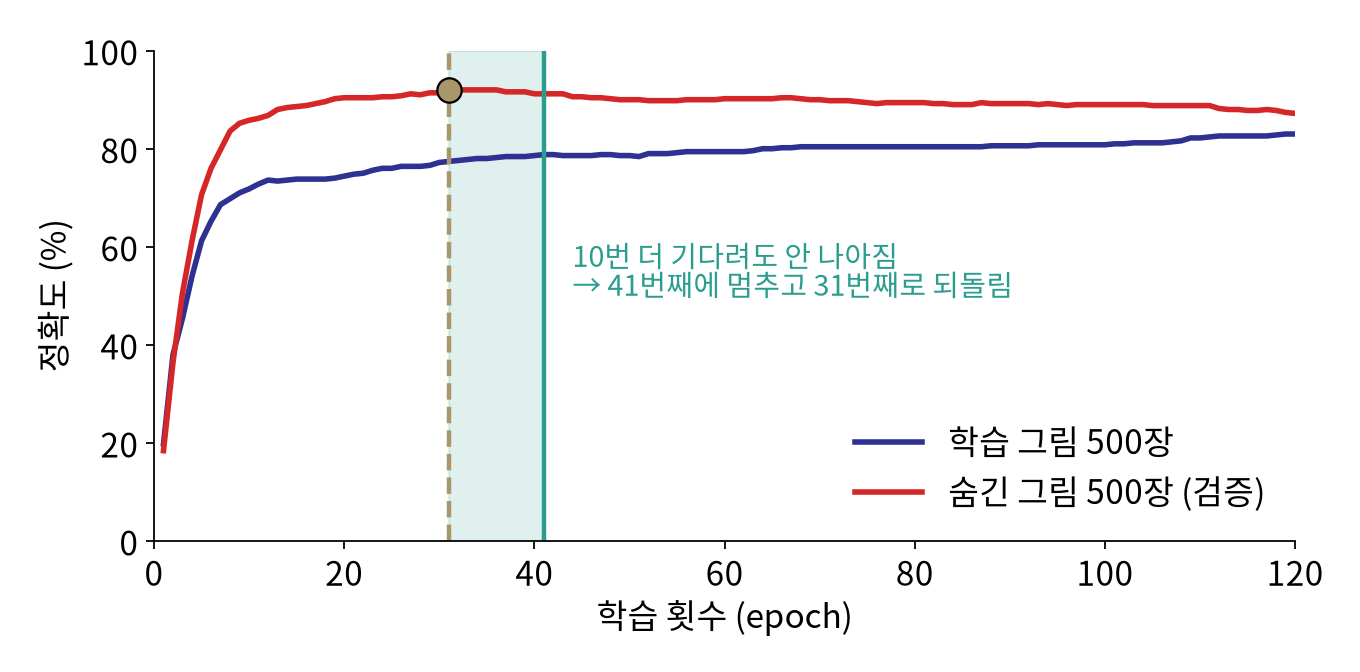
\includegraphics[width=0.6\linewidth]{es_patience.png}\par\vskip0.2em
{\large \textbf{참을성 (patience)} 만큼 더 기다려 보고 멈춘 뒤 \kb{최고였던 모델로 되돌린다}}\\[0.2em]
{\small 참을성 10: 31번째 최고 $\to$ 41번째까지 안 나아짐 $\to$ 멈추고 31번째 모델 (검증 92\%)}
\vfill
\note{그래서 검증 정확도가 가장 높을 때 멈춥니다. 이게 Early Stopping, 조기 종료입니다. 문제는 지금이 최고점인지는 지나 봐야 안다는 겁니다. 검증 정확도는 오르내리니까요. 그래서 최고 기록이 나온 뒤 정해진 횟수만큼 더 기다려 보고, 그동안 기록이 깨지지 않으면 멈춥니다. 이 기다리는 횟수를 참을성, patience라고 합니다. 참을성을 10으로 하면 31번째 최고 기록 뒤 41번째까지 나아지지 않아서 멈추고, 저장해 둔 31번째 모델로 되돌립니다.}
\end{frame}

% --- 알고리즘
\begin{frame}{알고리즘}
\vfill
\centering
{\large\begin{tabular}{rl}
1 & $\text{best} \leftarrow -\infty$, \quad $\text{wait} \leftarrow 0$\\
2 & 한 번 학습하고 검증 정확도 $a$ 를 잰다\\
3 & $a > \text{best}$ 이면: \; $\text{best} \leftarrow a$, \; 지금 모델을 \kb{저장}, \; $\text{wait} \leftarrow 0$\\
4 & 아니면: \; $\text{wait} \leftarrow \text{wait} + 1$, \quad $\text{wait} = \text{patience}$ 이면 \kq{멈춤}\\
5 & 2 로 돌아간다. 끝나면 \kb{저장한 모델}을 쓴다
\end{tabular}}\vskip0.8em
{\small Keras \texttt{EarlyStopping(patience=10, restore\_best\_weights=True)}, scikit-learn \texttt{MLPClassifier(early\_stopping=True)}}
\vfill
\note{알고리즘으로 쓰면 이렇습니다. 최고 기록과 기다린 횟수를 기록해 둡니다. 한 번 학습할 때마다 검증 정확도를 재서, 최고 기록을 깨면 기록을 바꾸고 지금 모델을 저장하고 기다린 횟수를 0으로 되돌립니다. 못 깨면 기다린 횟수를 1 늘리고, 참을성만큼 기다렸으면 멈춥니다. 끝나면 저장해 둔 모델을 씁니다. 거의 모든 딥러닝 라이브러리에 이 기능이 들어 있습니다. Keras는 EarlyStopping 콜백, scikit-learn은 MLPClassifier의 early_stopping 옵션입니다.}
\end{frame}

% --- 참을성
\begin{frame}{참을성은 얼마나?}
\vfill
\centering
\renewcommand{\arraystretch}{1.3}
{\Large\begin{tabular}{cccc}
참을성 & 멈춘 번째 & 되돌린 번째 & 검증 정확도\\\hline
1 & 21 & 20 & \kq{90\%}\\
3 & 23 & 20 & \kq{90\%}\\
5 & 36 & 31 & \kb{92\%}\\
10 & 41 & 31 & \kb{92\%}\\
50 & 81 & 31 & \kb{92\%}
\end{tabular}}\vskip0.6em
{\large 짧으면 잠깐의 흔들림에 속아 \kq{일찍} 멈추고, 길면 시간만 더 든다 (결과는 같다)}
\vfill
\note{참을성을 바꿔 봤습니다. 1이나 3으로 짧게 하면 20번째 근처의 작은 봉우리 뒤에 잠깐 떨어진 것에 속아 일찍 멈추고, 검증 정확도가 90퍼센트에 그칩니다. 5 이상이면 31번째의 진짜 최고점까지 가서 92퍼센트를 얻습니다. 참을성을 50으로 길게 해도 결과는 같습니다. 최고 모델로 되돌리니까요. 대신 81번째까지 학습하느라 시간이 더 듭니다. 보통 5에서 20 사이를 씁니다.}
\end{frame}

% --- 정규화로서
\begin{frame}{학습 횟수도 손잡이다}
\vfill
\centering
\renewcommand{\arraystretch}{1.5}
{\large\begin{tabular}{lll}
손잡이 & 너무 작으면 & 너무 크면\\\hline
다항식 차수 (1주차) & 과소적합 & 과대적합\\
정규화 $\lambda$ (6주차) & 과대적합 & 과소적합\\
$k$ (kNN) & 과대적합 & 과소적합\\
\textbf{학습 횟수} & 과소적합 & \kq{과대적합}
\end{tabular}}\vskip0.8em
{\large 모두 \textbf{검증 데이터}로 고른다 \quad 조기 종료 = 학습 횟수를 검증으로 고르는 것}
\vfill
\note{학습 횟수도 지금까지 본 손잡이들과 같습니다. 다항식 차수, 정규화의 람다, kNN의 k처럼 너무 작아도 너무 커도 문제이고, 그 사이를 검증 데이터로 고릅니다. 학습 횟수가 적으면 아직 덜 배운 과소적합, 많으면 외워 버린 과대적합입니다. 조기 종료는 결국 학습 횟수라는 손잡이를 검증 데이터로 고르는 방법입니다. 그래서 정규화의 한 종류로 분류하기도 합니다. 신경망은 가중치가 너무 커지기 전에 멈추게 되니 효과도 릿지와 비슷합니다.}
\end{frame}

% --- 주의
\begin{frame}{주의: 멈춘 시점도 검증 데이터를 본 결과다}
\vfill
\centering
{\Large 검증 정확도 92\% 는 \kq{조금 낙관적}이다}\\[0.8em]
{\large 300개 시점 중 검증에서 가장 잘 나온 것을 골랐으니까}\\[0.8em]
{\large $\to$ 최종 성능은 학습에도, 멈추기에도 쓰지 않은 \kb{시험 데이터}로 한 번}
\vfill
\note{하나 주의할 점이 있습니다. 31번째에서 멈춘 것도 검증 데이터를 보고 정한 결정입니다. 300개 시점 중 검증에서 가장 잘 나온 걸 골랐으니, 검증 정확도 92퍼센트에는 운이 조금 섞여 있습니다. 지난 시간에 test로 여러 번 고르면 점수가 부풀려진다고 했던 것과 같은 이야기입니다. 그래서 최종 성능은 학습에도, 멈추는 시점 고르기에도 쓰지 않은 시험 데이터로 한 번 잽니다.}
\end{frame}

% --- 문제풀이
\begin{frame}{문제풀이}
\vfill
\begin{enumerate}
\item 검증 정확도가 1번째부터 80, 85, 88, 87, 89, 88, 88, 87 (\%) 이다. 참을성 2 이면 몇 번째에서 멈추고 어느 모델로 되돌리나? 참을성 3 이면?\vskip0.8em
\item 학습 정확도와 검증 정확도가 둘 다 계속 오르다가 300번째에 끝났다. 무엇을 의심해야 하나?\vskip0.8em
\item 조기 종료를 쓰는데 검증 데이터를 따로 두지 않고 학습 데이터 정확도로 멈추면 어떻게 되나?
\end{enumerate}
\vfill
\note{1번 답. 참을성 2면 3번째에 88로 최고, 4번째 87, 5번째 89로 다시 최고라 기다림이 리셋됩니다. 6번째 88, 7번째 88로 두 번 못 깨서 7번째에 멈추고 5번째 모델로 되돌립니다. 참을성 3이면 8번째 87까지 세 번 못 깨서 8번째에 멈추고 역시 5번째로 되돌립니다. 2번 답. 아직 덜 배운 과소적합일 수 있습니다. 더 학습해 보거나 학습률을 키워 봅니다. 3번 답. 학습 정확도는 거의 계속 오르니 멈추지 않거나 마지막까지 가서, 조기 종료의 효과가 없습니다.}
\end{frame}

% --- 실습
\begin{frame}{실습}
\vfill
\centering\begin{tabular}{rl}
\large 1 & 같은 실험 재현: 손글씨 500장 (정답 20\% 바꿈), 300번 학습 곡선\\[0.5em]
\large 2 & 참을성 있는 조기 종료 직접 구현 $\to$ 41번째에 멈추고 31번째로 되돌리기\\[0.5em]
\large 3 & 정답을 안 바꾸면? \; scikit-learn \texttt{early\_stopping=True} 와 비교
\end{tabular}\vskip1em
Optical Recognition of Handwritten Digits (Alpaydin \& Kaynak; UCI, scikit-learn \texttt{load\_digits}) \\[0.4em]\href{https://colab.research.google.com/github/SuminHan/book-ml/blob/main/slides/v2/ml1/week06/early_stopping/lab/early_stopping.ipynb}{\textcolor{ksagolddk}{▶ Colab에서 실습 노트북 열기}}
\vfill
\note{실습은 세 부분입니다. 첫째, 오늘의 실험을 그대로 재현해서 학습 곡선을 그립니다. 둘째, 참을성 있는 조기 종료를 반복문으로 직접 구현해서 41번째에 멈추고 31번째 모델로 되돌립니다. 셋째, 정답을 바꾸지 않은 깨끗한 데이터에서는 곡선이 어떻게 다른지 보고, scikit-learn에 들어 있는 early_stopping 옵션과 비교합니다.}
\end{frame}

% --- 정리
\begin{frame}{정리}
\vfill
\centering\large\begin{tabular}{l}
오래 학습하면 학습 정확도는 오르지만 \kq{검증 정확도는 떨어질 수 있다} (92 $\to$ 83\%)\\[0.5em]
이유: 예외와 실수까지 외운다 (틀린 정답 2장 $\to$ 86장)\\[0.5em]
\textbf{Early Stopping}: 검증 최고점에서 멈춤, \textbf{참을성}만큼 기다리고 최고 모델로 되돌림\\[0.5em]
학습 횟수도 손잡이 $\to$ 검증으로 고르고, 최종 성능은 시험 데이터로
\end{tabular}
\vfill
\note{정리합니다. 오래 학습하면 학습 정확도는 계속 오르지만, 검증 정확도는 오늘처럼 92에서 83퍼센트로 떨어질 수 있습니다. 데이터 속의 예외와 실수까지 외우기 때문입니다. 조기 종료는 검증 정확도가 가장 높을 때 멈추는 방법이고, 최고점은 지나 봐야 알기 때문에 참을성만큼 기다린 뒤 최고였던 모델로 되돌립니다. 학습 횟수도 차수나 람다 같은 손잡이라서 검증으로 고르고, 최종 성능은 시험 데이터로 잽니다.}
\end{frame}
\end{document}
